\documentclass{../lab_class}

\usepackage{fancyhdr}
\pagestyle{fancy}
\rhead{П.\,Ю. Смирнов, 687 гр.}
\lhead{Лабораторная работа № 3.3.2, МФТИ, осень 2017}

\begin{document}

{\Large 3.3.2 -- Исследование вольт-амперной характеристики вакуумного диода.}

\paragraph{Цель работы.}
Определение удельного заряда электрона на основе закона <<трёх вторых>>.
В работе используются: вакуумный диод, микроамперметр, вольтметр, стабилизированные источники тока.

\paragraph{Теоретическая часть.}

\begin{wrapfigure}[12]{r}{4cm}
\centering
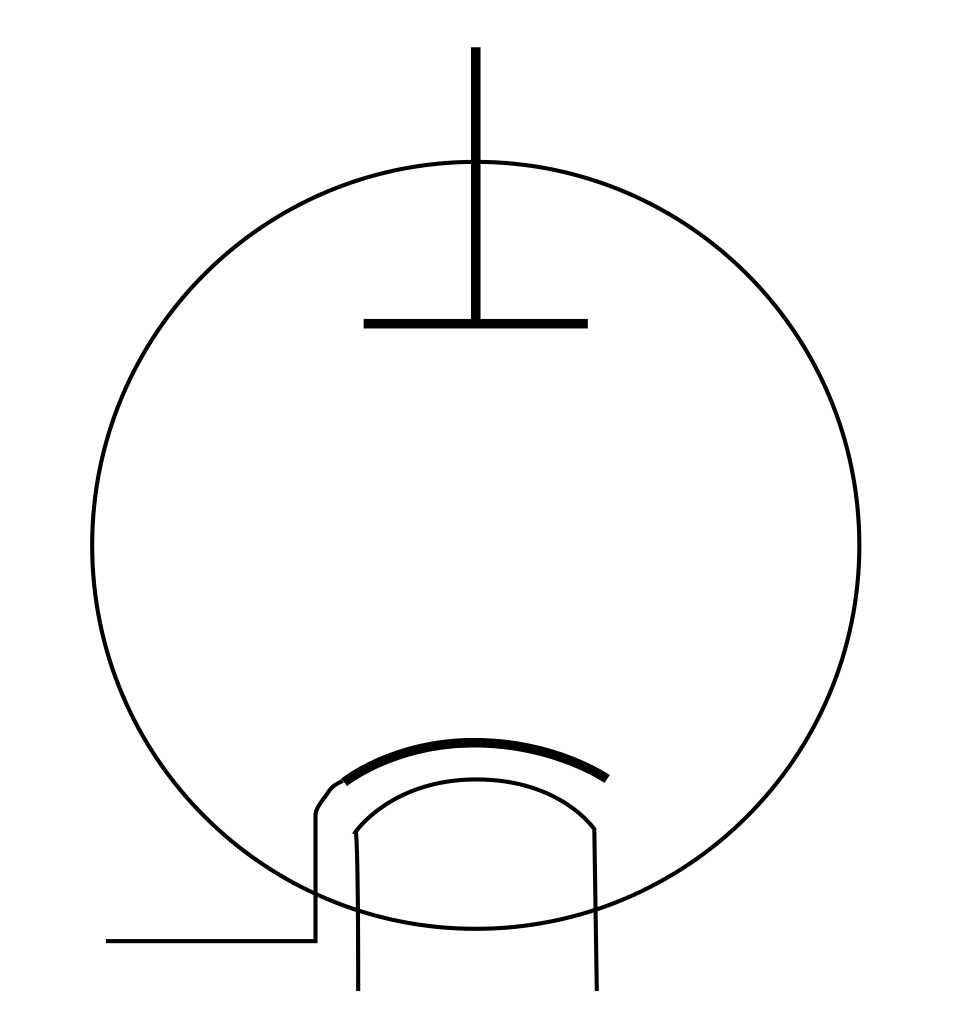
\includegraphics[width=3cm]{vacuum_diode.png}
\caption{Схема вакуумного диода}
\end{wrapfigure}

В основе работы вакуумного диода лежит явление термоэлектронной эмиссии, при которой электрон совершает работу выхода с поверхности твердого тела за счёт кинетической энергии теплового движения. Диод имеет простое устройство и состоит из двух частей -- катода и анода. На катод подается некоторый ток, называемый \emph{током накала}, за счёт которого он нагревается и эмитирует электроны. Между катодом и анодом подается постоянное напряжение, иными словами, создается постоянное электрическое поле, увлекающее к аноду эмитированные электроны -- возникает электрический ток. При постоянной температуре катода количество эмитируемых в единицу времени электронов постоянно, благодаря чему при некотором напряжении $U_{\text{нас}}$ возникает эффект насыщения. Более того, сила тока зависит от напряжения отнюдь не по линейному закону, поскольку поток электронов в пространстве между катодом и анодом создает некоторое дополнительное электрическое поле. Эта зависимость имеет степенной характер и называется \emph{законом <<трёх вторых>>}:
\begin{equation}
	I = c V^{\frac{3}{2}}.
\end{equation}

Приведём её упрощенный вывод. Рассмотрим плоский диод (см. рисунок), направим ось $x$ перпендикулярно катоду в сторону анода. Тогда суть задачи сводится к решению одномерного уравнения Пуассона
\begin{equation}
	\dv[2]{\varphi}{x} = - \frac{\rho}{\varepsilon_0}.
\end{equation}
Плотность тока есть $j = \rho v$, скорость электронов определим из уравнения $\frac{m v^2}{2} = e \varphi$. При этом мы считаем, что потенциал катода нулевой, и пренебрегаем начальными тепловыми скоростями. Отсюда имеем дифференциальное уравнение
\begin{equation*}
	\dv[2]{\varphi}{x} = \sqrt{\frac{m}{2e\varphi}} j
\end{equation*}
с начальными условиями $\varphi(0) = 0$ и $\dv{\varphi}{x} (0) = 0$. Отсюда получаем
\begin{equation}
	I = \frac{4 \varepsilon_0 S}{9 d^2} \sqrt{\frac{2e}{m}} V^{\frac{3}{2}},
\end{equation}
где $d$ -- расстояние между электродами, а $S$ -- площадь катода. Мы видим, что исследование вольт-амперной характеристики вакуумного диода позволят нам определить удельный заряд электрона!

Оказывается, указанная степенная зависимость $I(V)$ не зависит от геометрии диода, а вот постоянный множитель ещё как. Решение похожей (малоинтересной) задачи для используемого в нашей лаборатории цилиндрического диода даёт следующий результат:
\begin{equation}\label{eq:main_f}
	I = \frac{8\sqrt{2}\pi\varepsilon_0 l}{9} \sqrt{\frac{e}{m}} \frac{1}{r_a \beta^2} V^{\frac{3}{2}},
\end{equation}
где $r_a$ -- радиус анода, $l$ -- расстояние между электродами, $\beta^2$ -- некая волшебная функция, возникающая при решении дифференциального уравнения. 

\paragraph{Результаты эксперимента.}

\begin{wrapfigure}[12]{l}{11cm}
\centering
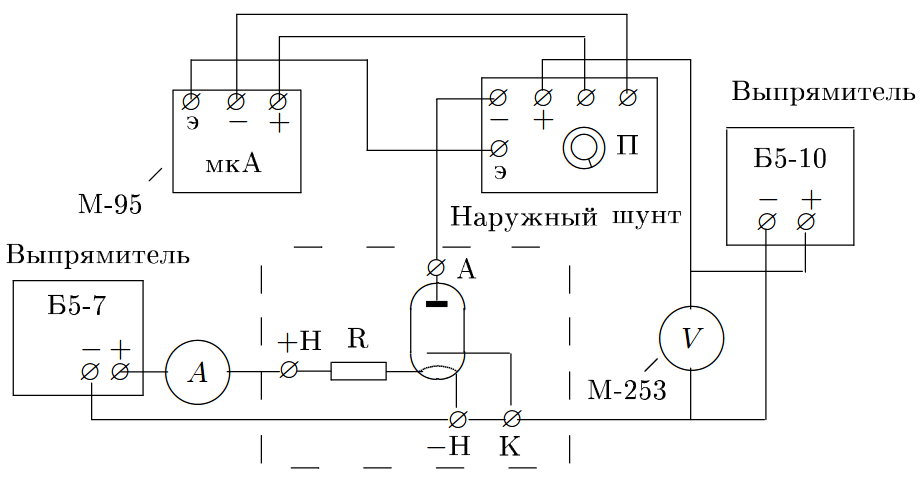
\includegraphics[width=8cm]{lab_scheme.png}
\caption{Схема экспериментальной установки}
\end{wrapfigure}

Исследование проводилось на диоде \verb|2Ц2С|, его параметры: $l = 9 \mm$, $r_a = 9.5 \mm$, $\beta^2 = 0.98$. Схема экспериментальной установки на рисунке. Вольт-амперная характеристика снималась для разных значений тока накала; впрочем, влияния температуры катода на результат эксперимента не наблюдается. Для каждого значения тока строим график $I=f(V^{\frac{3}{2}})$ и строим линейную аппроксимацию; иными словами, мы ищем зависимость в виде $I = k V^{\frac{3}{2}}$.

\bigskip

\begin{table}[H]
\centering
\begin{tabular}{|c|c|c|c|c|c|c|c|}
\hline
\multicolumn{2}{|c|}{$I_{\text{нак}}$ = 1.3 \A}	& \multicolumn{2}{c|}{$I_{\text{нак}}$ = 1.4 \A} &\multicolumn{2}{c|}{$I_{\text{нак}}$ = 1.5 \A} &\multicolumn{2}{c|}{$I_{\text{нак}}$ = 1.6 \A}\\ \hline
$I$, \smu \A &$U$, \V	&$I$, \smu \A &$U$, \V &$I$, \smu \A &$U$, \V &$I$, \smu \A &$U$, \V \\ \hline
3.88	&0.5	&6.74	&0.5	&13.1	&0.5	&23.2	&0.5	\\ \hline
12.39	&1		&16.71	&1		&25.8	&1		&37.1	&1		\\ \hline
22.78	&1.5	&28.81	&1.5	&41.7	&1.5	&56.7	&1.5	\\ \hline
38.34	&2		&44.2	&2		&59.4	&2		&75.2	&2		\\ \hline
54.5	&2.5	&62.8	&2.5	&79.4	&2.5	&95.4	&2.5	\\ \hline
72.6	&3		&82.5	&3		&95.4	&3		&117	&3		\\ \hline
90.7	&3.5	&102.2	&3.5	&123.7	&3.5	&142	&3.5	\\ \hline
111		&4		&126	&4		&145	&4		&166	&4		\\ \hline
134		&4.5	&148.6	&4.5	&165	&4.5	&194	&4.5	\\ \hline
156.1	&5		&174.1	&5		&196	&5		&221	&5		\\ \hline
183		&5.5	&198	&5.5	&223	&5.5	&246	&5.5	\\ \hline
205		&6		&226	&6		&249	&6		&278	&6		\\ \hline
261.5	&7		&283	&7		&309	&7		&339	&7		\\ \hline
320		&8		&344	&8		&378	&8		&410	&8		\\ \hline
390		&9		&413	&9		&446	&9		&480	&9		\\ \hline
454		&10		&485	&10		&556	&10		&598	&10		\\ \hline
893		&15		&942	&15		&990	&15		&1045	&15		\\ \hline
1400	&20		&1468	&20		&1535	&20		&1600	&20		\\ \hline
2006	&25		&2090	&25		&2160	&25		&2242	&25		\\ \hline
2663	&30		&2755	&30		&2850	&30		&2943	&30		\\ \hline
3368	&35		&3484	&35		&3589	&35		&3690	&35		\\ \hline
4136	&40		&4265	&40		&4393	&40		&4502	&40		\\ \hline
4954	&45		&5192	&45		&5324	&45		&5448	&45		\\ \hline
5896	&50		&6090	&50		&6235	&50		&6372	&50		\\ \hline
\end{tabular}
\caption{Экспериментальные данные.}
\end{table}

\begin{figure}[H]
\centering
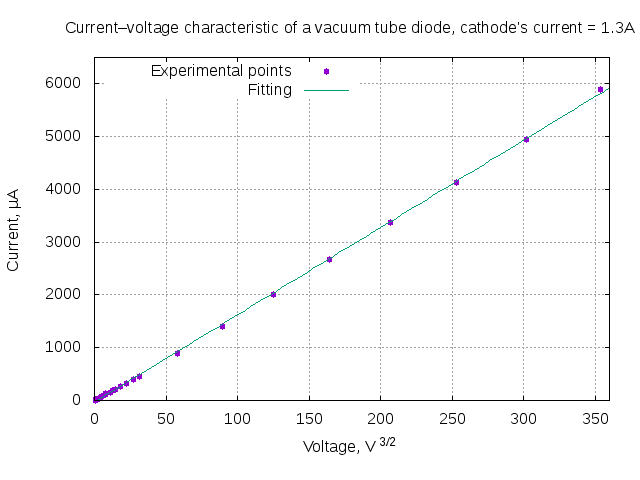
\includegraphics[width = 0.87 \textwidth]{graph_i13.png}
\caption{$I_{\text{нак}}$ = 1.3 \A, $k = 16.54 \pm 0.06 \ \smu\A / \V^\frac{3}{2}$.}
\end{figure}

\begin{figure}[H]
\centering
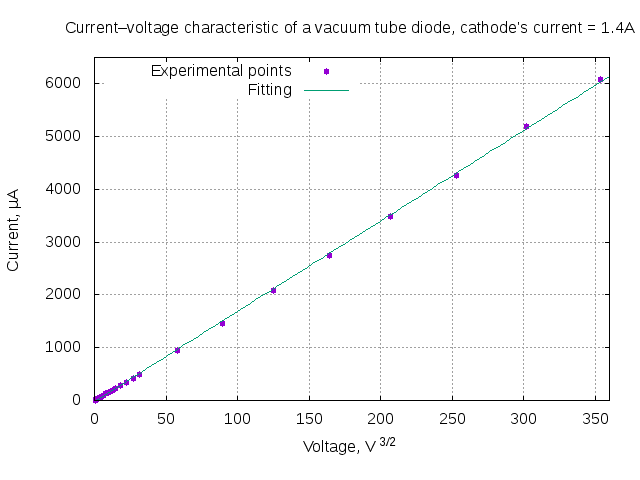
\includegraphics[width = 0.87 \textwidth]{graph_i14.png}
\caption{$I_{\text{нак}}$ = 1.4 \A, $k = 17.13 \pm 0.05 \ \smu\A / \V^\frac{3}{2}$.}
\end{figure}

\begin{figure}[H]
\centering
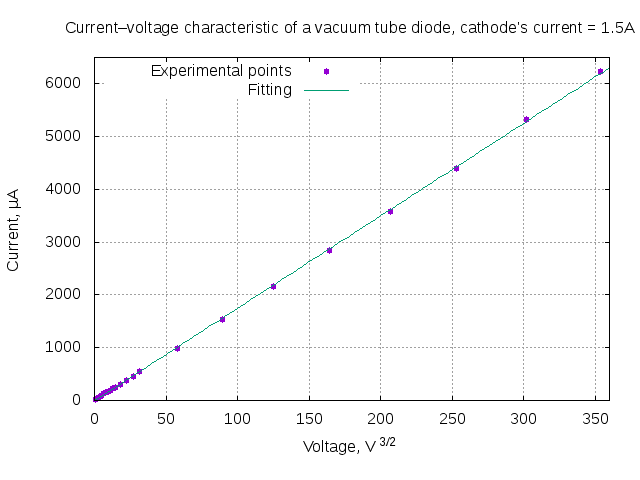
\includegraphics[width = 0.87 \textwidth]{graph_i15.png}
\caption{$I_{\text{нак}}$ = 1.5 \A, $k = 17.53 \pm 0.04 \ \smu\A / \V^\frac{3}{2}$.}
\end{figure}

\begin{figure}[H]
\centering
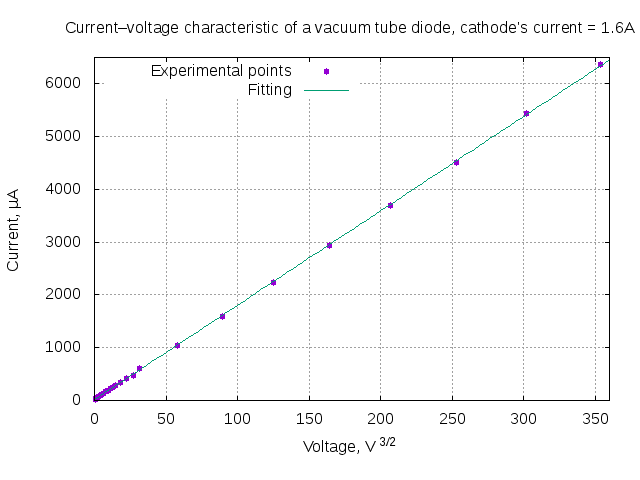
\includegraphics[width = 0.87 \textwidth]{graph_i16.png}
\caption{$I_{\text{нак}}$ = 1.6 \A, $k = 17.89 \pm 0.03 \ \smu\A / \V^\frac{3}{2}$.}
\end{figure}

Усредняя результаты, мы получаем значение удельного заряда электрона, используя формулу $\ref{eq:main_f}$:
\begin{gather*}
	k = 17.27 \pm 0.04 \ \smu\A / \V^\frac{3}{2} \then \frac{e}{m} = (2.4 \pm 0.6) \times 10^{11} \ \text{Кл} / {\kg}.
\end{gather*}
Заметим, что табличное значение удельного заряда составляет $1.7 \times 10^{11} \ \text{Кл} / {\kg}$; таким образом, наш метод дает вполне приемлемую точность.

\paragraph{Вывод.}
Справедливость закона <<трёх-вторых>> проверена экспериментально для частного случая геометрии вакуумного диода. Показано, как данный метод может быть использован для измерения удельного заряда электрона; полученные данные в пределах точности измерений хорошо соответствуют известным табличным значениям.

\end{document}